\section{Excitación sísmica}
\label{sec:excitacion}

Hasta esta etapa se utilizó un martillo instrumentado PCB 086D20 como fuente y como
referencia temporal del impacto. Su elemento de cuarzo ICP entrega
\SI{0.23}{\milli\volt\per\newton}, admite picos de \SI{22.24}{\kilo\newton} y presenta
una resonancia igual o superior a \SI{12}{\kilo\hertz}. Estas prestaciones permiten
registrar la fuerza aplicada sin introducir otro sensor en la interfaz mecánica
\cite{PCB086D20}.

El 086D20 requiere entre \SIrange{20}{30}{\volt} y una excitación de corriente constante
de \SIrange{2}{20}{\milli\ampere}; su salida queda superpuesta a una polarización de
\SIrange{8}{14}{\volt}. PCB recomienda una fuente regulada, un elemento de corriente
constante y un capacitor de desacople que elimine esa componente continua antes de la
adquisición \cite{PCBSignalConditioning}.

El acondicionador se integró en el PSoC. Un convertidor eleva los \SI{5}{\volt} de USB a
\SI{21}{\volt}; el LM7805, usado como regulador de corriente con \SI{1}{\kilo\ohm},
entrega del orden de \SI{5}{\milli\ampere} al martillo. Un capacitor de
\SI{47}{\micro\farad} bloquea la polarización ICP y la señal alterna pasa por PGA,
pasa-bajos y ADC $\Delta\Sigma$. De esta forma la fuerza de impacto se registra en la
misma plataforma y puede alinearse con las respuestas de los geófonos.

En paralelo se desarrolla un martillete inspirado en un mecanismo de leva. El diseño
conceptual eleva y libera repetidamente la masa para producir trenes de impulsos con
repetición controlada. Hasta ahora se construyeron el bastidor y el conjunto preliminar
formado por motor y martillo; quedan por integrar la transmisión, el guiado, el control
y las protecciones antes de realizar ensayos. El objetivo es mejorar la repetibilidad y
concentrar energía por debajo de la obtenida con un único golpe manual.

\begin{figure*}[!t]
\centering
\begin{minipage}[c]{0.18\textwidth}
\centering
\textbf{(a) 086D20 empleado}\par\smallskip
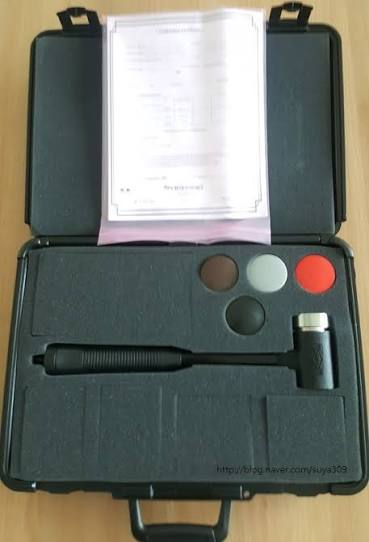
\includegraphics[height=0.13\textheight,keepaspectratio]{figuras/excitacion/martillo_086d20.png}
\end{minipage}
\hfill
\begin{minipage}[c]{0.24\textwidth}
\centering
\textbf{(b) Diseño conceptual del martillete}\par\smallskip
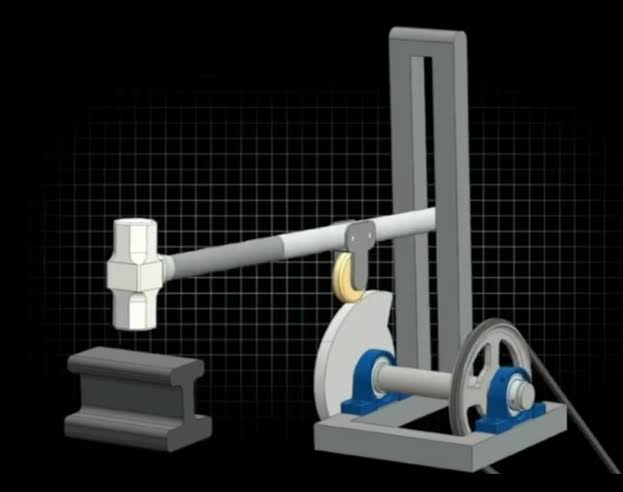
\includegraphics[width=0.94\textwidth]{figuras/excitacion/concepto_martillete_da_vinci.png}
\end{minipage}
\hfill
\begin{minipage}[c]{0.53\textwidth}
\centering
\textbf{(c) Estado actual del prototipo}\par\smallskip
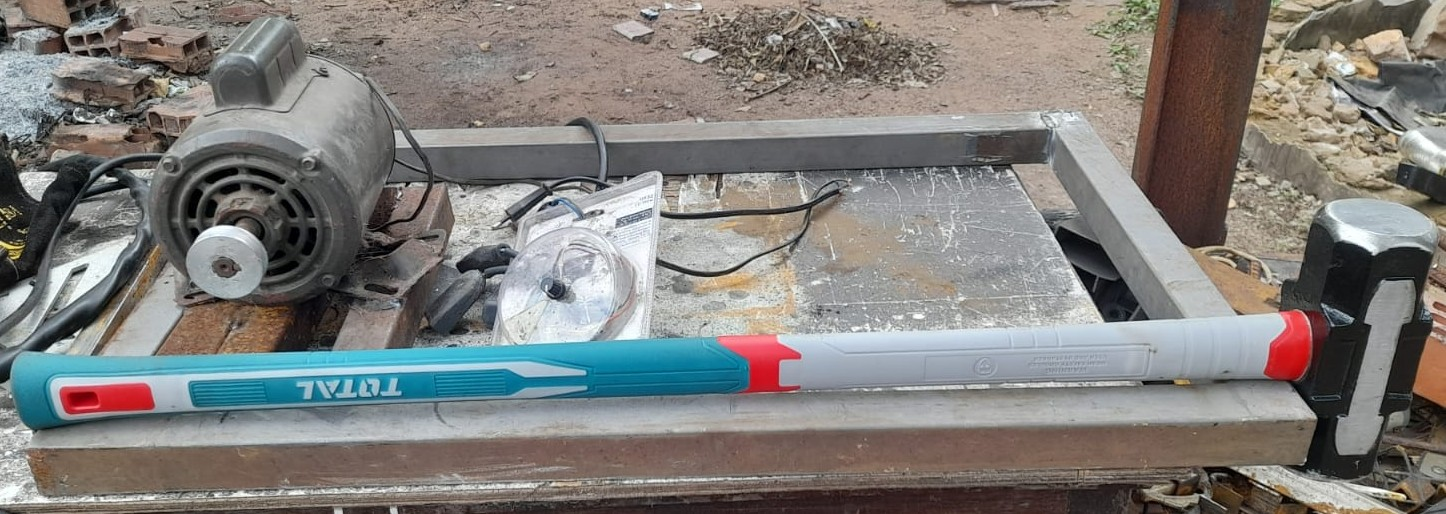
\includegraphics[width=\textwidth]{figuras/excitacion/estado_actual_martillete.jpg}
\end{minipage}

\medskip
\begin{minipage}[c]{0.32\textwidth}
\centering
\textbf{(d) Principio ICP}\par\smallskip
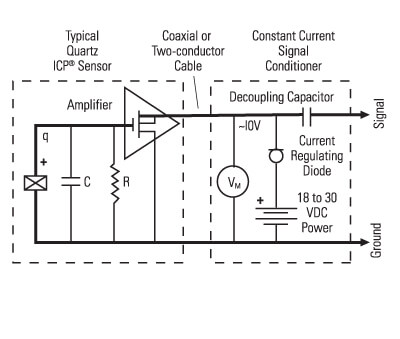
\includegraphics[width=\textwidth]{figuras/excitacion/principio_icp_corriente_constante.png}
\end{minipage}
\hfill
\begin{minipage}[c]{0.64\textwidth}
\centering
\textbf{(e) Acondicionamiento implementado en el PSoC}\par\smallskip
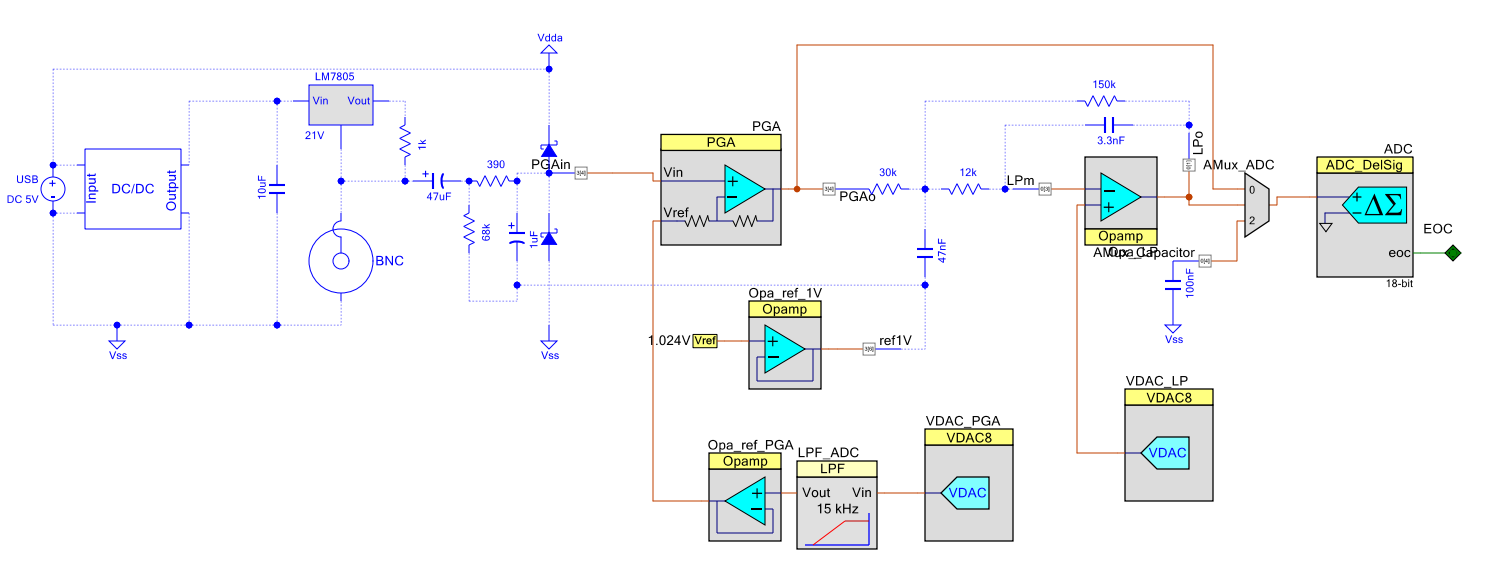
\includegraphics[width=\textwidth]{figuras/excitacion/acondicionamiento_martillo_psoc.png}
\end{minipage}
\caption{Excitación sísmica. (a) Martillo instrumentado utilizado. (b) Diseño
conceptual del martillete. (c) Estado actual: bastidor, motor y martillo antes de
integrar transmisión, guiado y control. (d) Alimentación y desacople ICP recomendados
por PCB. (e) Fuente de corriente con LM7805, acondicionamiento y ADC implementados.}
\label{fig:acondicionamiento-martillo-davinci}
\end{figure*}
\FloatBarrier
